\documentclass[journal]{vgtc}                % final (journal style)
%\documentclass[review,journal]{vgtc}         % review (journal style)
%\documentclass[widereview]{vgtc}             % wide-spaced review
%\documentclass[preprint,journal]{vgtc}       % preprint (journal style)
%\documentclass[electronic,journal]{vgtc}     % electronic version, journal

%% Uncomment one of the lines above depending on where your paper is
%% in the conference process. ``review'' and ``widereview'' are for review
%% submission, ``preprint'' is for pre-publication, and the final version
%% doesn't use a specific qualifier. Further, ``electronic'' includes
%% hyperreferences for more convenient online viewing.

%% Please use one of the ``review'' options in combination with the
%% assigned online id (see below) ONLY if your paper uses a double blind
%% review process. Some conferences, like IEEE Vis and InfoVis, have NOT
%% in the past.

%% Please note that the use of figures other than the optional teaser is not permitted on the first page
%% of the journal version.  Figures should begin on the second page and be
%% in CMYK or Grey scale format, otherwise, colour shifting may occur
%% during the printing process.  Papers submitted with figures other than the optional teaser on the
%% first page will be refused.

%% These three lines bring in essential packages: ``mathptmx'' for Type 1
%% typefaces, ``graphicx'' for inclusion of EPS figures. and ``times''
%% for proper handling of the times font family.

\usepackage{mathptmx}
\usepackage{graphicx}
\usepackage{times}

%% We encourage the use of mathptmx for consistent usage of times font
%% throughout the proceedings. However, if you encounter conflicts
%% with other math-related packages, you may want to disable it.

% declare the path(s) where your graphic files are
\graphicspath{{Figure/}{Images/}{../../Images/}}
% and their extensions so you won't have to specify these with
% every instance of \includegraphics
\DeclareGraphicsExtensions{.pdf,.jpg,.png}

%---------------------------------------------------
\usepackage[cmex10]{amsmath}
\usepackage{amssymb}
\usepackage{color}
% \usepackage[dvipsnames,svgnames]{xcolor}
% \usepackage{ulem}
% \usepackage[section]{placeins}
\usepackage[caption=false,font=footnotesize,labelfont=sf,textfont=sf]{subfig}
% \usepackage{sidecap}
\usepackage{multirow}
\usepackage{bbm}
\usepackage{url}
\usepackage{xr}
\usepackage{xr-hyper}
\usepackage{afterpage}


\usepackage{todonotes}
\newcommand{\hhnote}[1]{\todo[inline,color=magenta!40]{#1}}

%---------------------------------------------------

%% This turns references into clickable hyperlinks.
\usepackage[bookmarks,backref=section,linkcolor=black]{hyperref} %,colorlinks
\hypersetup{
  pdfauthor = {},
  pdftitle = {},
  pdfsubject = {},
  pdfkeywords = {},
  colorlinks=true,
  linkcolor= black,
  citecolor= black,
  pageanchor=true,
  urlcolor = black,
  plainpages = false,
  linktocpage
}

\externaldocument{appendix}

%% If you are submitting a paper to a conference for review with a double
%% blind reviewing process, please replace the value ``0'' below with your
%% OnlineID. Otherwise, you may safely leave it at ``0''.
\onlineid{0}

%% declare the category of your paper, only shown in review mode
\vgtccategory{Theory/Model}

%% allow for this line if you want the electronic option to work properly
\vgtcinsertpkg

%% In preprint mode you may define your own headline.
%\preprinttext{To appear in IEEE Transactions on Visualization and Computer Graphics.}

%% Paper title.

\title{Spatial Reasoning and Data Displays}

%% This is how authors are specified in the journal style

%% indicate IEEE Member or Student Member in form indicated below
\author{Susan VanderPlas, and Heike Hofmann, \textit{Member, IEEE}}
\authorfooter{
%% insert punctuation at end of each item
\item Susan VanderPlas is a graduate student at Iowa State University. Email: skoons@iastate.edu.
\item Heike Hofmann is Professor of Statistics at Iowa State University and member of the faculty in the Human Computer Interaction program. Email: hofmann@iastate.edu.
}


%other entries to be set up for journal
\shortauthortitle{VanderPlas \MakeLowercase{\textit{et al.}}: Spatial Reasoning and Data Displays}
%\shortauthortitle{Firstauthor \MakeLowercase{\textit{et al.}}: Paper Title}


%% Abstract section.
\abstract{
Graphics convey numerical information very efficiently, but rely on a different set of mental processes than tabular displays. This study examines the demographic characteristics and visual skills associated with perception of graphical lineups. We conclude that lineups are essentially a classification test in a visual domain, and that performance on the lineup protocol is associated with general aptitude, rather than specific tasks such as card rotation and spatial manipulation. We also examine the possibility that specific graphical tasks may be associated with certain visual skills and conclude that more research is necessary to understand which visual skills are required in order to understand certain plot types. 
} % end of abstract

%% Keywords that describe your work. Will show as 'Index Terms' in journal
%% please capitalize first letter and insert punctuation after last keyword
\keywords{Data visualization, Perception, Statistical graphics, Statistical computing.}

%% ACM Computing Classification System (CCS). 
%% See <http://www.acm.org/class/1998/> for details.
%% The ``\CCScat'' command takes four arguments.

\CCScatlist{ % not used in journal version
 \CCScat{H.2.8.c}{Data and knowledge visualization}%
{Database applications}{Database management};
 \CCScat{G.3.n}{Statistical Computing}{Probability and Statistics}{Mathematics of Computing}
}

%% Uncomment below to include a teaser figure.
   \teaser{
    \centering
\begin{minipage}[c]{.5\textwidth}
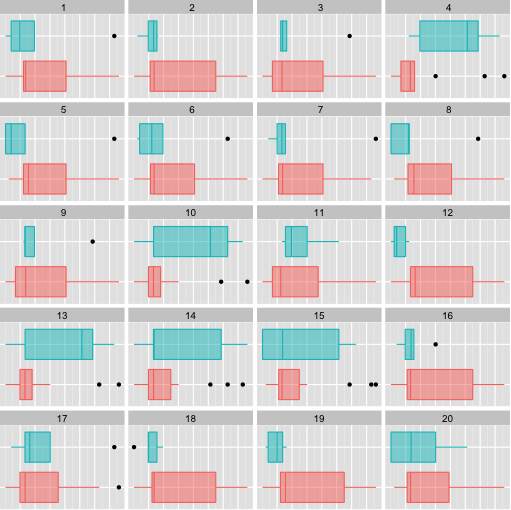
\includegraphics[width=\textwidth]{lineup}
\end{minipage}
\begin{minipage}[c]{.3\textwidth}
    \includegraphics[height=.8\textwidth]{Figure/fig-biplots-pca5-1}
    \includegraphics[height=.8\textwidth]{Figure/fig-biplots-pca5-2}
\end{minipage}
    \caption[Sample Lineup]{``Which of these plots is the most different from the others?"\newline
    This is the question participants are asked to answer for each of the lineups in the study. In the figure, a sample lineup of boxplots is shown. %Participants are instructed to choose the plot which appears most different from the others. 
    Panel 4 is the target plot, because the two groups have a large difference in medians.\label{fig:lineup}
    The plots on the right show biplots of principal components 2-5 with observations. The lineup task appears to be most similar to the figure classification task, based on the plot of PC2 vs. PC3.}
  }




%% Uncomment below to disable the manuscript note
%\renewcommand{\manuscriptnotetxt}{}

%% Copyright space is enabled by default as required by guidelines.
%% It is disabled by the 'review' option or via the following command:
% \nocopyrightspace

%%%%%%%%%%%%%%%%%%%%%%%%%%%%%%%%%%%%%%%%%%%%%%%%%%%%%%%%%%%%%%%%
%%%%%%%%%%%%%%%%%%%%%% START OF THE PAPER %%%%%%%%%%%%%%%%%%%%%%
%%%%%%%%%%%%%%%%%%%%%%%%%%%%%%%%%%%%%%%%%%%%%%%%%%%%%%%%%%%%%%%%%

\begin{document}

%% The ``\maketitle'' command must be the first command after the
%% ``\begin{document}'' command. It prepares and prints the title block.

%% the only exception to this rule is the \firstsection command
\firstsection{Introduction}

\maketitle

\label{sec:introduction}Data displays provide quick summaries of data, models, and results, but not all displays are equally good, nor is any data display equally useful to all viewers. 
Graphics utilize higher-bandwidth visual pathways to encode information~\cite{baddeley1974working}, allowing viewers to quickly and intuitively relate multiple dimensions of numerical quantities.
Well-designed graphics emphasize and present important features of the data while minimizing  features of lesser importance, guiding the viewer towards conclusions that are meaningful in context and supported by the data while maximizing the information encoded in working memory. Under this framework, well-designed graphics reduce memory load and make more cognitive resources available for other tasks (such as drawing conclusions from the data), at the cost of depending on certain visuospatial reasoning abilities. 

Many theories of graphical learning center around the difference between visual and verbal processing: the dual-coding theory emphasizes the utility of complementary information in both domains, while the visual argument hypothesis emphasizes that graphics are more efficient tools for providing data with spatial, temporal, or other implicit ordering, because the spatial dimension can be represented graphically in a more natural manner~\cite{vekiri2002value}. Both of these theories suggest spatial ability impacts a viewer's use of graphics, because spatial ability either influences cognitive resource allocation or affects the processing of spatial relationships between graphical elements. In addition, previous investigations into graphical learning and spatial ability have found relationships between spatial ability and the ability to read information from graphs~\cite{lowrie2007solving}. 
However,  mathematical ability, not spatial ability, was shown~\cite{shah1995conceptual} to be associated with accuracy on a simple two-dimensional line graph. 
Spatial ability becomes more important when more complicated graphical displays are used in comparison tasks: the lower performance of individuals with low spatial ability on tests utilizing diagrams and graphs is attributed ~\cite{mayer1994whom} to the fact that more cognitive resources are required to process the visual stimuli, which leaves fewer resources to make connections and draw conclusions from those stimuli. It is theorized that graphics are a form of ``external cognition"~\cite{scaife1996external} that guide, constrain, and facilitate cognitive behavior~\cite{zhang1997nature}. 

Here, we want to investigate the extent to which observers make use of spatial ability in their evaluation of and reasoning about statistical graphics. As a quantitative measure of how successful an evaluation is, we are making use of the lineup protocol  \cite{buja2009statistical, wickham2010graphical, majumder2013validation}. 

``Lineups" have recently been introduced as a tool to evaluate the statistical significance of a graphical finding. Lineups are also useful in assessing the effectiveness of different graphical displays \cite{hofmann2012graphical, loy:2015}. Like their police counterpart, lineups consist of several distractor plots (of randomly generated data) and one target (the data plot). 
% 
% \begin{figure}[htp]
% 
% \end{figure}

Figure~\ref{fig:lineup} shows a sample lineup of boxplots; participants are expected to identify the most different among the plots shown. In this example, sub-plot 4 is the target  because of the noticeably different locations of the two boxplot medians.


%This method is described in more detail in the next section; here we motivate the importance of understanding the connection between lineups and spatial reasoning. 


Lineups provide a quantitative measurement of the effectiveness of a particular plot: if participants consistently identify the target plot rather than the randomly-generated distractors, the plot effectively shows the difference between real data and random noise. 
This removes much of the subjectivity from user evaluations of display effectiveness, and the procedure is simple enough that it does not generally require participants to be very familiar with data-based graphics. 
While previous research~\cite{lowrie2007solving,mayer1994whom} has examined the link between certain types of graphical perception and spatial skills, it is important to identify any additional visual skills participants utilize to complete the lineup task, as well as better understand demographic characteristics (math education, research experience, age, gender) which may impact performance \cite{humanfactorslineups}. 

In this paper, we present the results of a study designed to compare lineup performance with visual aptitude and reasoning tests, examining the skills necessary to successfully evaluate lineups. 
We compare lineup performace to the visual search task (VST), paper folding test, card rotation test, and figure classification test. 
The VST measures visual search speed\cite{goldstein1973validity}, the paper folding and card rotation tests measures spatial manipulation ability, and the figure classification test measures inductive reasoning\cite{ekstrom1976manual}; 
all of these skills are at least peripherally recruited during the lineup task, but some may dominate in predicting performance on the lineup task. 
We hope to facilitate comparison of the lineup task to known cognitive tests, inform the design of future studies, and better understand the perception of statistical lineups. 


In section \ref{sec:methods} we introduce the tests used in the study and describe how the tests are scored. In section \ref{sec:results} we discuss the study results and compare them with scores previously established test, that also take  demographic characteristics associated with test scores into account. We discuss multi-collinearity in the study results, and use principal components analysis and linear models to draw some conclusions about the similarity between lineups and aptitude tests. Finally, in section \ref{sec:discussion}, we discuss the implications of the study results for the lineup protocol and  possible extensions. 


\section{Methods}\label{sec:methods}

\subsection{The Lineup Protocol}
The lineup protocol~\cite{hofmann2012graphical,wickham2010graphical, buja2009statistical} is a testing framework that allows researchers to quantify the statistical significance of a graphical finding with the same mathematical rigor as conventional hypothesis tests.

In a lineup test, the plot of the data is placed randomly among a set of, generally 19, distractor plots (or {\it null plots}) that are rendered from data generated by a model, without a signal (a null model). This sheet of charts is then shown to human observers, who are asked to identify the display that is ``the most different". If an observer identifies the plot drawn from the actual data, this can be reasonably taken as evidence that the data it shows is different from the data of other plots.
Let $X$ be the number of observers (out of $n$) who identify the data plot from the lineup. Under the null hypothesis that the data plot is not different from the other plots, $X$ has approximately a Binomial distribution \cite{wickham2010graphical, majumder2013validation}. If $k$ of the observers identify the data plot from the lineup, the probability $P(X \ge k)$ is the $p$-value of the corresponding visual test. 
%
By aggregating responses from different individuals the lineup protocol therefore allows an objective evaluation of a graphical finding. 

Additionally, however, we can aggregate the scores from the same individual on several lineups to objectively assess an individual's performance on the lineup task. 

For this approach, we derive a score for an individual as follows:

Assume that an observer has evaluated $K$ lineups of size $m$ (consisting of $m-1$ decoy plots and 1 target), and successfully identified the target in $n_c$ of these plots, while missing the target in $n_w$ of them. 
The score for this individual is then given as:
\begin{eqnarray}\label{eq.scoring1}
n_c - \frac{n_w}{m-1}.
\end{eqnarray}
Note that the sum of answers, $n_c + n_w$, is at most $K$, but may be less, if an observer chooses to not answer one of the lineup tasks or runs out of time.

The scoring scheme as given in (\ref{eq.scoring1}) is chosen so that if participants are guessing, the expected score is 0. 

Statistical lineups depend on the ability to search for a signal amid a set of distractors (visual search) and the ability to infer patterns from stimuli (pattern recognition). Depending on the choice of plot shown in the lineup, the task of identifying the most different plot might require additional abilities from   participants, e.g.~ polar coordinates depend on the ability to mentally rotate stimuli (spatial rotation) and mentally manipulate graphs (spatial rotation and manipulation). By breaking the lineup task down into its components, we  determine which visuospatial factors most strongly correlate with lineup performance, using carefully chosen cognitive tests to assess these aspects of visuospatial ability. 

Demographic factors are known to impact lineup performance: country, education, and age affected score on lineup tests, and all of those factors plus gender had an effect on the amount of time spent on lineups \cite{humanfactorslineups}. In addition, lineup performance can be partially explained using statistical distance metrics \cite{distancemetriclineups}, but these metrics do not completely succeed in predicting human performance, in part due to the difficulty of representing human visual ability algorithmically.


One of the most useful features of the lineup protocol is that it allows researchers to conclusively determine which graphics show certain features more conclusively by providing an experimental protocol for comparing graphics based on the accuracy of user conclusions. In addition, lineups provide researchers with a rigorous framework for determining whether a specific graph shows a real, statistically significant effect by comparing a target plot with plots formed using permutations of the same data, providing a randomization test protocol for graphics. As a result, lineups are a useful and innovative tool for evaluating charts; on an individual level, they can also be used to evaluate a specific participant's perceptual reasoning ability in the context of statistical graphics.


\subsection{Measures of visuospatial ability}

Participants are asked to complete several cognitive tests designed to measure spatial and reasoning ability. Tasks are timed such  that participants are under  pressure to complete; participants are not expected to finish all of the problems in each section. This allows for a better discrimination between scores and prevents score compression at the top of the range. 

The \textbf{visual searching task} (VST), shown in figure~\ref{fig:VST}, is designed to test a participant's ability to find a target stimulus in a field of distractors, thus making the visual search task similar in concept to lineups. Historically, visual search has been used as a measure of brain damage \cite{goldstein1973validity,demita1981validity,moerland1986neuropsychological}; however, similar tasks have been used to measure cognitive performance in a variety of situations, for example under the influence of drugs in~\cite{anderson1983interactive}. The similarity to the lineup protocol as well as the simplicity of the test and its' lack of color justify the slight deviation from forms of visual search tasks typically used in normal populations. 

\begin{figure}[htp]\centering
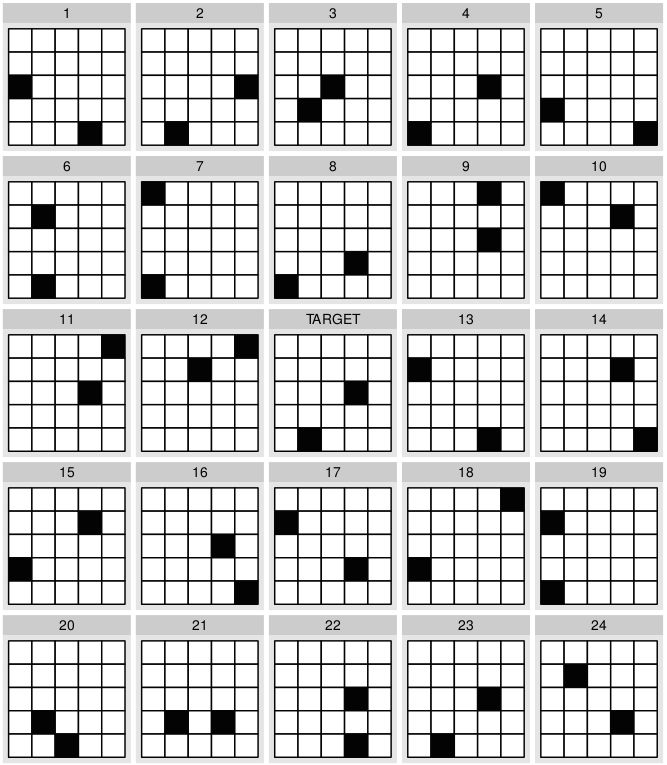
\includegraphics[width=.8\linewidth]{VisualSearch}
\caption[Visual Search Task]{Visual Search Task (VST). Participants are instructed to find the plot numbered 1-24 which matches the plot labeled ``Target". Participants will complete up to 25 of these tasks in 5 minutes.}\label{fig:VST}
\end{figure}

The \textbf{figure classification task} tests a participant's ability to extrapolate rules from provided figures. This task is associated with inductive reasoning abilities (factor I  in~\cite{ekstrom1976manual}). An example is shown in figure~\ref{fig:figureclassification}. 

The figure classification test requires the same type of reasoning as the lineups: participants must determine the rules from the provided classes, and extrapolate from those rules to classify new figures. In lineups, participants must determine the rules based on the panels appearing in the lineup; they must then identify the plot which does not conform. As such, the figure classification test has content validity in relation to lineup performance: it is measuring similar underlying criteria. 

The \textbf{card rotation test} measures a participant's ability to rotate objects in two dimensions in order to distinguish between left-hand and right-hand versions of the same figure. It tests mental rotation skills, and is classified as a test of spatial orientation in~\cite{ekstrom1976manual}, though it does require that participants have both mental rotation ability and short-term visual memory. An example is shown in figure~\ref{fig:cardrotation}. 
The card rotation test is often used in studies investigating the effect of visual ability on the use of visual aids \cite{mayer1994whom} and statistical graphs \cite{lowrie2007solving} in education.

Two-dimensional comparisons are an important component of lineup performance. In some lineup situations, these comparisons sometimes involve translation, but in other lineups, rotation is required. Lineups also require visual short-term memory, so the additional factor measured implicitly by this test does not reduce its potential relevance to lineup performance.  

The \textbf{paper folding test} measures participants' ability to visualize and mentally manipulate figures in three dimensions. A sample question from the test is shown in figure~\ref{fig:paperfolding}. It is classified as part of the visualization factor in~\cite{ekstrom1976manual}, which differs from the spatial orientation factor because it requires participants to visualize, manipulate, and transform the figure~mentally, which makes it a more complex and demanding task than simple rotation. The paper folding test is associated with the ability to extrapolate symmetry and reflection over multiple steps.

\begin{figure}[ht]
  \centering
   \subfloat[Figure Classification Task. Participants classify each figure in the second row as belonging to one of the groups above. Participants complete up to 14 of these tasks (each consisting of 8 figures to classify) in 8 minutes.\label{fig:figureclassification}]{%
  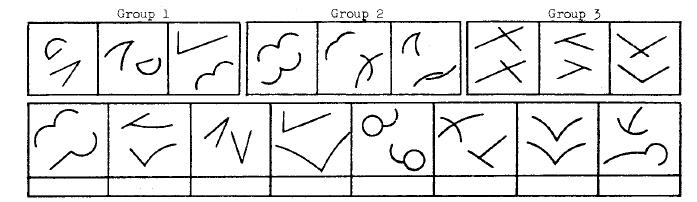
\includegraphics[width=.8\linewidth]{figureclassification}
}
\hfill
    \subfloat[Card Rotation Task. Participants mark each figure on the right hand side as either the same as or different than the figure on the left hand side of the dividing line. Participants complete up to 20 of these tasks (each consisting of 8 figures) in 6 minutes.\label{fig:cardrotation}]{%

\includegraphics[width=.8\linewidth]{cardrotation}
    }
    \hfill
    \subfloat[Paper Folding Task. Participants are instructed to pick the figure matching the sequence of steps shown on the left-hand side. Participants  complete up to 20 of these tasks in 6 minutes.\label{fig:paperfolding}]{%
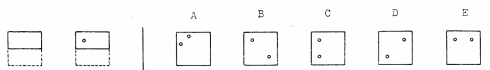
\includegraphics[width=.8\linewidth]{paperfolding}
   }
    \caption{Visuospatial tests}
    \label{fig:tests}
\end{figure}

Lineups require similar manipulations in two-dimensional space, and also require the ability to perform complex spatial manipulations mentally; for instance, comparing the interquartile range of two boxplots as well as their relative alignment to a similar set of two boxplots in another panel.

Between cognitive tasks, participants were also asked to complete three blocks of 20 lineups each, assembled from previous studies~\cite{hofmann2012graphical,majumder2013validation}. Participants were given 5 minutes to complete each block of 20 lineups. Figure~\ref{fig:lineup} shows a sample lineup of box plots. 

In addition to these tests, participants were asked to complete a questionnaire which includes questions about colorblindness, mathematical background, self-perceived verbal/mathematical/artistic skills, time spent playing video games, and undergraduate major. 
These questions are designed to assess different factors which may influence a participant's skill at reading graphs and performing spatial tasks. 

\subsection{Test Scoring}\label{sec:scaling}

All test results were scored so that random guessing produces an expected value of 0; therefore each question answered correctly contributes to the score by 1, while a wrong answer is scored by $-1/(k-1)$, where $k$ is the total number of possible answers to the question. Thus, for a test consisting of multiple choice questions with $k$ suggested answers with a single correct answer each, the score is calculated as
\begin{eqnarray}\label{eq.scoring}
\# \text{correct answers } - 1/(k-1) \cdot \# \text{wrong answers}.
\end{eqnarray}
This allows us to compare each participant's score in light of how many problems were attempted as well as the number of correct responses. Combining accuracy and speed into a single number does not only make a comparison of test scores easier,  this scoring mechanism is also used on many standardized tests, such as the SAT and the battery of psychological tests~\cite{diamond1973correction, ekstrom1976manual} from which parts of this test are drawn. The advantage of using tests from the Kit of Factor Referenced Cognitive tests~\cite{ekstrom1976manual} is that the tests are extremely well studied (including an extensive meta-analysis in~\cite{voyer1995magnitude} of the spatial tests we are using in this study) and comparison data are available from the validation of these factors~\cite{schaie1998longitudinal,hampson1990variations,mayer1994whom} and previous versions of the kit~\cite{educational1963kit}.

\section{Results}\label{sec:results}
Results are based on an evaluation of 38 undergraduate students at Iowa State University. 61\% of the participants were in STEM fields, the others were distributed relatively evenly between agriculture, business, and the social sciences. Students were evenly distributed by gender, and were between 18 and 24 years of age with only one exception. This is reasonably representative\footnote{\url{http://www.registrar.iastate.edu/sites/default/files/uploads/stats/university/F14summary.pdf}} of the university as a whole; in the fall 2014 semester, 26\% of students were associated with the college of engineering, 24\% were associated with the college of liberal arts and sciences, 15\% were associated with the college of human sciences, 7\% with the college of design, 13\% with the business school, and 15\% with the school of agriculture.  

\subsection{Comparison of Spatial Tests with Previously Validated Results}
The card rotation, paper folding, and figure classification tests have been validated using different populations, many of which are demographically similar to Iowa State students (naval recruits, college students, late high-school students, and 9th grade students). We compare Iowa State students' unscaled scores in Table~\ref{tab:scorecomparison}, adjusting data from other populations to account for subpopulation structure and test length. 


\begin{table*}[htb]\centering
\begin{tabular}{rlllc}
\hline
  & Card Rotation & Paper Folding & Figure Classification & Visual Search  \\\hline
ISU Students & 83.4 (24.1) 
             & 12.4 (3.7)
             & 57.0 (23.8)\footnotemark[1]
             & 21.9 (2.3)\\
Scaled Scores & 88.0 (34.8)
              & 13.8 (4.5)
              & 58.7 (14.4)\footnotemark[2]
              & -- \\
Unscaled Scores & 44.0 (24.6)\footnotemark[3]
                & 13.8 (4.5)
                & \parbox[c]{.2\linewidth}{M:~120.0~(30.0)\\ F:~114.9~(27.8)}
                & --\\\hline
{\footnotesize Population}    
              & \parbox[t]{.15\linewidth}{\footnotesize approx.\ 550 male\\ naval recruits} 
              & \parbox[t]{.17\linewidth}{\footnotesize 46 college students\\(1963~version)}
              & \parbox[t]{.2\linewidth}{\footnotesize suburban 11th \& 12th \\ grade students\\(288-300 M, 317-329 F)}
              & \\\hline
\end{tabular}
\caption[Comparison of scores for cognitive tasks.]{Comparison of scores from Iowa State students and scores reported in~\protect\cite{ekstrom1976manual}. Scaled scores are calculated based on information reported in the manual, scaled to account for differences in the number of questions answered during this experiment. Data shown are from the population most similar to ISU students, out of the data available. The visual search task~\protect\cite{goldstein1973validity,demita1981validity,moerland1986neuropsychological} is not part of the Kit of Factor Referenced Cognitive Test data, and thus we do not have comparison data for the form used in this experiment.
\label{tab:scorecomparison}}
\end{table*}

Table~\ref{tab:scorecomparison} shows mean scores and standard deviation for ISU students and other populations. Values have been adjusted to accommodate for differences in test procedures and sub-population structure; for instance,  some data is reported for a single part of a two-part test, or results are reported for each gender separately (adjustment procedure is described in more detail in Appendix~\ref{app:ScoreAdj}). Once these adjustments have been completed, it is evident that Iowa State undergraduates scored at about the same level as other similar demographics. In fact, both means and standard deviations of ISU students' scores are similar to the comparison groups, which were chosen from available demographic groups based on population similarity. 

Comparison population data was chosen to most closely match ISU undergraduate population demographics. Thus, if comparison data was available for 9th and 12th grade students, scores of Iowa State students were compared to scores of 12th grade students, who are closer in age to college students. When data was available from college students and Army enlistees, comparisons of scores were based on other college students, as college students are more likely to have a similar gender distribution to ISU students.

Applying the grading protocol discussed in section~\ref{sec:scaling}, we see that the ranges of lineup and visuospatial test scores do not include zero; this indicates that we do not see random guessing from participants in any task. Figure~\ref{fig:Scores} shows the range of possible scores and the observed score distribution. 
Participants' scores on the VST indicate score compression; that is, both participants with medium and high visual search abilities scored at the extremely high end of the spectrum. 
In future experiments, participants should be given less time (or more questions) to better differentiate participants with medium and high-ability.


\begin{figure}[ht]
\centering
\includegraphics[width=.9\linewidth]{Figure/fig-ResultsScaledScores-1}
\caption{Test scores for lineups and visuospatial tests. As none of the participants scored at or below zero, we can conclude that there is little evidence of random guessing. We also note the score compression that occurs on the Visual Search test; this indicates that most participants scored extremely high, and thus, participants' scores are not entirely representative of their ability. \label{fig:Scores}}
\end{figure}
% 
%\afterpage{\clearpage}

% Applying the grading protocol discussed in section~\ref{sec:scaling}, we see that the ranges of lineup and visuospatial test scores do not include zero; this indicates that we do not see random guessing from participants in any task. Figure~\ref{fig:Scores} shows the range of possible scores and the observed score distribution. 


\subsection{Lineup Performance and Demographic Characteristics}


\begin{figure*}[h!tb]\centering
\includegraphics[width=.85\linewidth]{fig-VisReasoningCategorical-1}
\caption[Visual Aptitude Study Results]{Demographic characteristics of participants compared with lineup score. Categories are ordered by effect size; majoring in a STEM field, calculus completion, hours spent playing video games per week, and sex are all associated with a significant difference in lineup score. }\label{fig:visualaptitudecat}
\end{figure*}
%\afterpage{\clearpage}

%Next, we examine the effect of demographic factors on lineup performance. 
Previous work found a relationship between lineup performance and demographic factors such as education level, country of origin, and age \cite{humanfactorslineups}; our participant population is very homogeneous, which allows us to explore factors such as educational background and skills on performance in lineup tests. 

Figure~\ref{fig:visualaptitudecat} shows participants' lineup scores in relationship to their responses in the questionnaire given at the beginning of the study; this allows us to explore effects of demographic characteristics (major, research experience, etc.) on test performance. 

Completion of Calculus I is associated with increased performance on lineups; this may be related to general math education level, or it may be that success in both lineups and calculus requires certain visual skills. This association is consistent with findings in~\cite{shah1995conceptual}, which associated  mathematical ability to performance on simple graph description tasks.  There is also a significant relationship between hours of video games played per week and score on lineups, however, this association is not monotonic and the groups do not have equal sample size, so the conclusion may be suspect. There is a (nearly) significant difference between male and female performance on lineups; this is not particularly surprising, as men perform better on many spatial tests~\cite{voyer1995magnitude} and performance on spatial tests is correlated with phase of the menstrual cycle in women~\cite{hausmann2000sex}. There is no significant difference in lineup performance for participants of different age, self-assessed skills in various domains, previous participation in math or science research, completion of a statistics class, or experience with AutoCAD. These demographic characteristics were chosen to account for life experience and personal skills which may have influenced the results. Statistical test results are available in Appendix~\ref{app:categoricalresults}. 

\subsection{Understanding Visual Abilities and Lineup Performance}



\begin{figure}[ht]
\centering
\includegraphics[width=.9\linewidth]{Figure/fig-VisReasoningSPM-1}
\caption{Pairwise scatterplots of test scores. Lineup scores are most highly correlated with figure classification scores, and are also highly correlated with card rotation scores. Paper folding and card rotation scores are also highly correlated.\label{fig:scatterplotmatrix}}
\end{figure}
%\afterpage{\clearpage}



Results from the visuospatial tests used in this experiment are highly correlated, as shown in Figure~\ref{fig:scatterplotmatrix}; this is to be expected given that all of these tests are in some way measuring individuals' visual ability. 
What is of more interest to us is how other factors, such as e.g.~general intelligence, mental processing speed, cognitive resources, motivation, and attention affect performance. 
In order to assess factors contributing to lineup performance, we first examine the separate dimensions measured by the battery of cognitive tests (other than lineups) using principal components analysis on the scaled test scores, then we examine all five tests using the same procedure. 


A principal component analysis (PCA) of the four established visuo-spatial tests reveals that they all share a very strong first component, which explains about 64\% of the total variability. Principal components (PC-) are ordered by importance (how much variability in the data they contain), and each principal component is uncorrelated with every other principal component. 

PC1 is essentially an average across all tests representing a general ``visual intelligence" factor. The other principal components span another two dimensions, while the last dimension is weak (at 6\%). 
PC2 differentiates the figure classification test from the visual searching test, whereas PC3 differentiates these two tests from the paper folding test. 
% More detailed results from the 4-test analysis are provided in Appendix~\ref{app:pca}.

% latex table generated in R 3.1.1 by xtable 1.7-3 package
% Mon Mar 30 14:32:39 2015
\begin{table}[htb]
\centering
\caption{Importance of principal components in an analysis of four tests of spatial ability: figure classification, paper folding, card rotation, and visual search.\label{tab:PCAvariance4}} 
{\footnotesize
\begin{tabular}{rrrrr}
  \hline
 & PC1 & PC2 & PC3 & PC4 \\ 
  \hline
Standard deviation & 1.61 & 0.81 & 0.73 & 0.49 \\ 
  Proportion of Variance & 0.64 & 0.16 & 0.13 & 0.06 \\ 
  Cumulative Proportion & 0.64 & 0.81 & 0.94 & 1.00 \\ 
   \hline
\end{tabular}
}
\end{table}

Table~\ref{tab:PCAvariance4} contains the proportion of the variance in the four cognitive tasks represented by each principal component. PC1 accounts for about 60\% of the variance; Figure~\ref{fig:biplots4} and Table~\ref{tab:PCArotation4} confirm that PC1 is a measure of the similarity between all 4 tests; that is, a participant's general (or visual) aptitude. PC2 differentiates the figure classification test from the visual searching test, while PC3 differentiates these two from the paper folding test. PC4 is not particularly significant (it accounts for 5.9\% of the variance), but it differentiates the card rotation task from the paper folding task.

% latex table generated in R 3.1.1 by xtable 1.7-3 package
% Mon Mar 30 14:32:39 2015
\begin{table}[htb]
\centering
\caption{Rotation matrix for principal component analysis of the four cognitive tests (visual search, paper folding, card rotation, figure classification).\label{tab:PCArotation4}} 
\begin{tabular}{rrrrr}
  \hline
 & PC1 & PC2 & PC3 & PC4 \\ 
  \hline
card.rot & 0.55 & -0.19 & -0.38 & 0.72 \\ 
  fig.class & 0.46 & 0.58 & 0.66 & 0.14 \\ 
  folding & 0.52 & 0.33 & -0.53 & -0.59 \\ 
  vis.search & 0.46 & -0.72 & 0.38 & -0.34 \\ 
   \hline
\end{tabular}
\end{table}




















